%#!platex --src-specials main.tex
\chapter{考察}
\label{chap:cons}
本章では実験結果に対する考察を述べる. 
\section{次元削減の有無による比較}
図\ref{fig:accuracy}, \ref{fig:precision}, \ref{fig:recall}, \ref{fig:fmeasure}より, 4つすべての評価指標において, 無加工の3軸加速度触覚データを入力に用いた場合の分類が最も高い値を記録している. 
特に精度において,  DFT321 で処理した触覚データの分類は76.5\%に比べ無加工の3軸加速度触覚データは96.9\%と20\%以上高い. 
また4つすべての指標において, 次点の高い値を示した手法よりも3\%程度かそれ以上の分類性能を有していることがわかる. 
これらから今回比較したいかなる次元削減手法も, CNN での分類において有意な情報が欠損してしまい, 精度に大きく影響すると言える. 
したがって, 分類精度の観点から見ると3軸加速度触覚データに対して CNN での分類を行う場合は得られた3軸加速度触覚データを次元削減せず入力として使用する手法が最も優れていると言える.

次元削減を行ったデータの中で比較を行うと, 無加工の1軸抽出を行うアルゴリズムである SA321 において軸ごとにばらつきがあるもののx軸を抽出する SA321-x が比較的良い値を記録している. これはテクスチャ分類の際に重要となる, 指でテクスチャをなぞる際の表面に対して鉛直方向の軸に比較的近い軸であった事が考えられる. 
また, DFT321 に関して, 精度, 再現率に関して他の手法に比べともに76.5\%と低い値であったが, 適合率に関しては92.9\%と比較的良い値を記録している. これは分類問題に対して, 予測したクラスが確実にそのクラスに分類される尺度である. これより DFT321 は複雑な前処理を施したため, テクスチャに対してより狭く顕著である特徴を中心に抽出, 学習してしまいその特徴に高いレベルで合致しなければ正しく分類ができないような現象が起きたことが推測される. 

また, 次元削減を行う主目的である計算量の削減に関して, それぞれのデータの前処理と学習にかかった時間を以下の図\ref{fig:process_time}に示す. 
図\ref{fig:process_time}より, 多少の差はあるが学習時間には有意差は無く, むしろ次元削減を施した PCA と DFT321 は明らかに無加工の3軸加速度データに比べ処理時間がかかっている. 
処理時間は使用するコンピュータ, ハードウェアにも大きく起因し単純な計算量の比較とは全く言えないが, 少なくとも CNN の学習に関して影響はほぼ与えないと考える. 

\begin{figure}[H]
    \begin{center}
    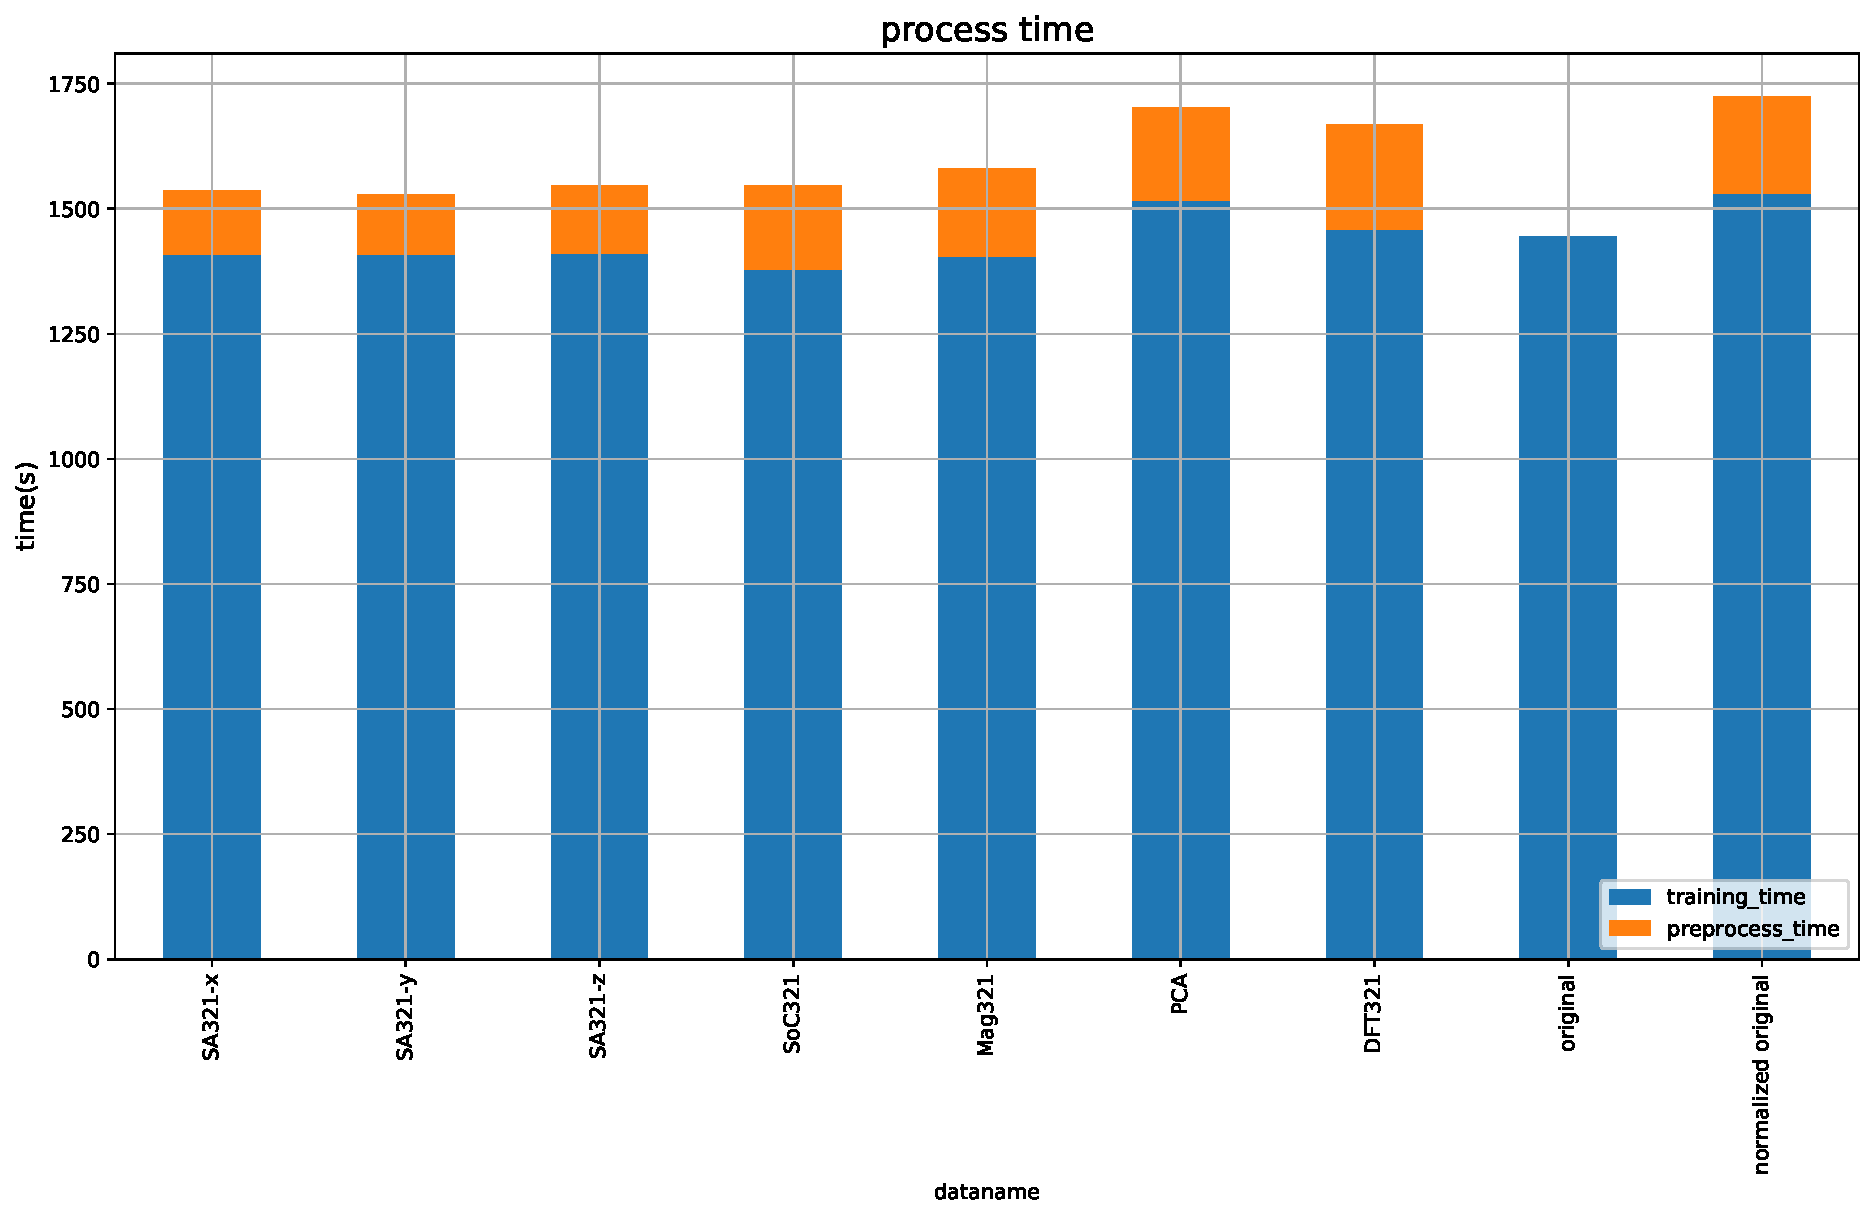
\includegraphics[width=12cm]{eps/process_time.pdf}
    \caption{各データ処理手法に対する前処理時間と学習時間}
    \label{fig:process_time}
   \end{center}
   \end{figure}
   
\section{正規化の有無による比較}
正規化の有無についても比較を行う. この比較に関しても4つすべての評価指標において, 無加工の3軸加速度触覚データを入力に用いた場合の分類が正規化を行った3軸加速度触覚データに比べ高い値を記録している. 
したがって, 分類精度の観点から見ると3軸加速度触覚データに対して CNN での分類を行う場合は得られた3軸加速度触覚データの正規化は有意ではないと言える.
正規化が分類に有利に働かなかった理由として, 3軸加速度のスケールがほぼ同じであることに起因すると考える. 
正規化はパラメータ間のスケールを統一しネットワークのパラメータによる更新幅の違いを吸収する役割を持つ. 
しかし3軸加速度データに関しては同一センサから得た3軸を3つのパラメータとして取り扱うのでスケールはほぼ同一な上, そこに付随するスケーリング前の値がクラス分類に有意な特徴となったと思われる. 
したがって正規化を行った際に特徴が一部消失し, 無加工の3軸加速度触覚データよりも低い分類精度を記録したと考える. 
% Local Variables:
% TeX-master: "main"
% mode: yatex
% End:
